\documentclass[10pt, xcolor=table, dvipsnames]{beamer}
\usepackage[scale=3]{beamerposter}
\setlength{\paperwidth}{72in} % A0 width: 46.8in
\setlength{\textwidth}{72in}
\setlength{\paperheight}{45 in} % A0 height: 33.1in
\setlength{\textwidth}{45 in}
\usepackage[overlay,absolute]{textpos}
\usepackage{tikz}
\usetikzlibrary{shapes,arrows, fit}
\usepackage{tcolorbox}
\tcbuselibrary{raster}
\usepackage{enumitem}
\setlist{label=\textbullet} 
\usepackage{multicol}
\usepackage{multirow}
\usepackage{booktabs}
\usepackage{longtable}
\usepackage{array}
\usepackage{multirow}
\usepackage{wrapfig}
\usepackage{float}
\usepackage{colortbl}
\usepackage{pdflscape}
\usepackage{tabu}
\usepackage{threeparttable}
\usepackage{threeparttablex}
\usepackage[normalem]{ulem}
\usepackage{makecell}
\usepackage{xcolor}
\TPGrid[20mm,20mm]{1}{1}
\tcbset{%
	noparskip,
	colback=white, %background color of the box
	colframe=black, %color of frame and title background
	coltext=black, %color of body text
	coltitle=black, %color of title text 
	colbacktitle=Violet!30,
	boxrule=4pt,
	fonttitle=\bfseries,
}
\usepackage{xcolor}
\usepackage{soul}
\makeatletter
\let\HL\hl
\renewcommand\hl{%
	\let\set@color\beamerorig@set@color
	\let\reset@color\beamerorig@reset@color
	\HL}
\makeatother
\usepackage{pifont}
\newcommand{\cmark}{{\color{ForestGreen}\ding{51}}}
\newcommand{\xmark}{{\color{red}\ding{55}}}%
\newcommand{\qmark}{{\color{blue}\textbf{?}}}%
\begin{document}
	\begin{textblock}{1}(0.0,0)
		\begin{tcolorbox}[colback=Violet!30]{}
			
			
			\begin{centering} 
				\bigskip
				
				{\LARGE\textbf{Communicative reduction in referring expressions \\ within a
						multi-player negotiation game}}\\
				{\Large Veronica Boyce, Michael C. Frank} \\
				{Stanford University, contact: vboyce@stanford.edu}	
				
			\end{centering}
		\end{tcolorbox}
	\end{textblock}
	
	\begin{textblock}{.32}(0,0.15)
		\begin{tcolorbox}[title= {\centering Goals }]
			\vspace{.5em}
			\begin{small}\centering
				\bigskip
			\textbf{The ability to form novel conventions is a key signature of efficient
			linguistic communication.}
			
			\vspace{.5em}
 In dyadic reference games (Clark \& Wilkes-Gibbs 1986, Hawkins et al. 2020), speaker-listener pairs show the following patterns:
 \begin{itemize}
 	\item \textbf{reduction} as utterances shorter over time,
 	 \item \textbf{convergence} within groups to a shared nickname,
 	  \item \textbf{divergence} between groups as different nicknames develop.
   \end{itemize}

\vspace{.5em}
\textbf{Do these patterns occur for reference expressions in strategic games with more complex goals?}
\vspace{.5em}


			\end{small}
		\end{tcolorbox}
	\end{textblock}
	
	

	\begin{textblock}{.32}[0,1](0,1 )
		\begin{tcolorbox}[title={\centering Experimental design }]
\vspace{.5em}
			
			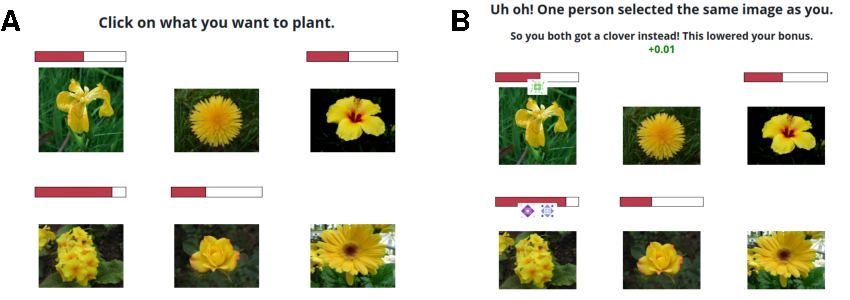
\includegraphics[clip,width=\textwidth]{interface-1.pdf}
			
			\vspace{.5em}
			\begin{small}
				
				Participants were assigned to 3-player games. 
				 During selection (A) each participant saw 6 flowers, 4 with value bars. Players could communicate in a chat box before each selecting a flower. Then they saw feedback (B) indicating who chose what.  When multiple players selected the same flower, they received a lower value rather than the indicated value. 

\vspace{.5em}

				In \emph{individual utility} games (18 games), each player earned points for the
				flowers they selected; in the \emph{shared utility} games (21 games), the points
				were averaged together, and all players in a game got the same reward.
								Each group played 24 trials with images drawn from a set of 12 flowers. This data was first presented in  Mankewitz et al. (2021).
								
							
								
			\end{small}
		
		\vspace{.5em}
		\end{tcolorbox}
	\end{textblock}
	
	
	\begin{textblock}{.41}[0,0](.33,.15)
	\begin{tcolorbox}[title={\centering Referring expressions reduced over time}]  
		\vspace{.5em}
		\centering
		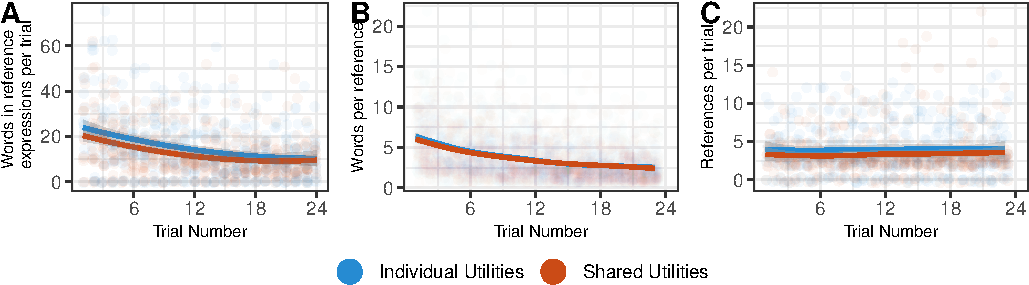
\includegraphics[width=.9\textwidth]{wordcount-1.pdf}    
		
	\begin{small}	Descriptions got shorter over time, but the number of descriptions stayed constant.   \end{small}                                              
	\end{tcolorbox}
\end{textblock}

	
		\begin{textblock}{.41}[0,0](.33,.4)

		\begin{tcolorbox}[title={\centering Referring expressions converged within groups}]  
			\vspace{.5em}
			\centering
			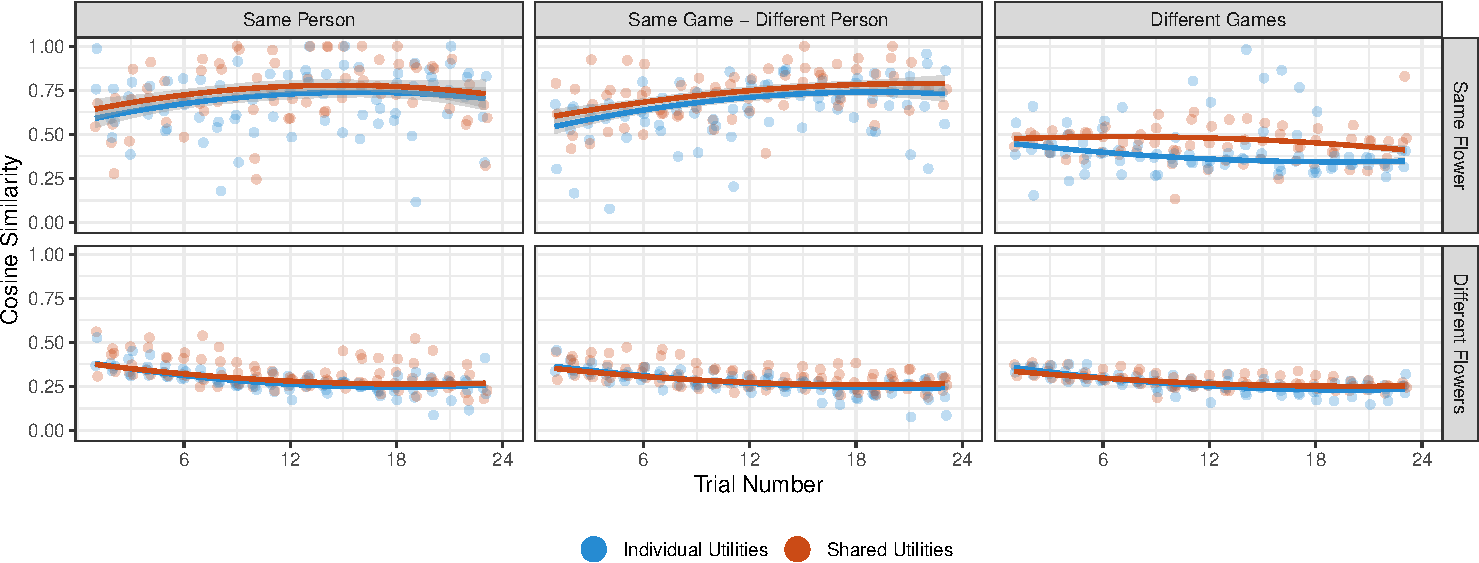
\includegraphics[width=.9\textwidth]{during-1.pdf}                            			                                                  
			\begin{small}
				
				
					Similarity between two descriptions was measured by the cosine between their S-BERT embeddings (Reimers \& Gurevych, 2019).
				\begin{itemize}

				\item Similarity increased for the same flower within games (top left, center). 
				
				\item Similarity decreased slightly for the same flower across games (top right). 
				
				\item Descriptions for different flowers became more distinct (bottom).
				\end{itemize}
			\end{small}
		\vspace{.5em}
		\end{tcolorbox}
	\end{textblock}


	\begin{textblock}{.41}[0,1](.33,1)
	\begin{tcolorbox}[title={ \centering 					Shared utilities games diverged less}]  
		\begin{minipage}{.4\textwidth}
			\vspace{.5em}
			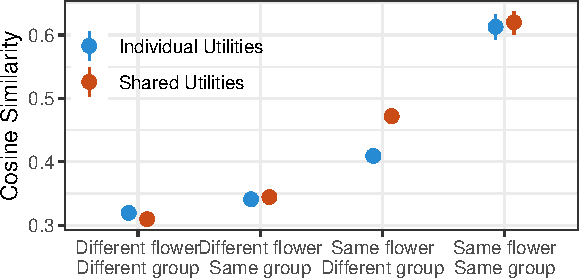
\includegraphics[width=\textwidth]{withinend-1.pdf}    
		\end{minipage}
	\hfill
	\noindent
	\begin{minipage}{.55\textwidth}
				\begin{small}
					\vspace{.5em}
			Shared utility games diverged less from each other in how to refer to each flower, both during game (above, top right) and in post-game descriptions (left), possibly due to the shared utilities encouraging coordination and thus comprehension.
				
				\vspace{.2em}
				\end{small}
			
	\end{minipage}

		
		                        			                                                  
	\end{tcolorbox}
\end{textblock}


		\begin{textblock}{.25}[1,0](1,.15)
	\begin{tcolorbox}[title={\centering Examples}]
		\vspace{.2em}
		
		\centering
		\begin{footnotesize}
			Descriptions of different flowers from different games. Images shown in  experimental design: flower 1 upper left, flower 2 lower center, flower 3 lower left.
			\vspace{-1em}
			
			\centering
			\begin{tabular}[t]{llr>{\raggedright\arraybackslash}p{16em}}
				\toprule
				Flower & Game & Trial & Expression\\
				\midrule
				1 & 1A & 2 & not sure what kind of flower it is but the droopy-ish one\\
				1 & 1C & 4 & droopy iris flower\\
				1 & 1B & 21 & droopy\\
				\midrule
				2 & 2B & 2 & the red middle with spike\\
				2 & 2B & 3 & the red center\\
				2 & 2A & 20 & red middle\\
				2 & 3C & 6 & the one with the dark red centre\\
				2 & 3A & 13 & the one with black background\\
				2 & 3A & 24 & black background\\
				\midrule
				3 & 1A & 4 & the big cluster of flowers with the orange in the middle\\
				3 & 1A & 23 & cluster\\
				3 & 2C & 24 & bundle\\
				3 & 3B & 24 & multi flowers\\
				\bottomrule
			\end{tabular}
			
			\vspace{1em}
			Cosine similarities between pairs of descriptions. 
			
			\vspace{-1.5em}
			\begin{tabular}[t]{>{\raggedright\arraybackslash}p{9em}>{\raggedright\arraybackslash}p{9em}r}
				\toprule
				Expression 1 & Expression 2 & Sim\\
				\midrule
				the red center & red middle & 0.78\\
				droopy iris flower & multi flowers & 0.56\\
				droopy iris flower & droopy & 0.56\\
				cluster & bundle & 0.25\\
				red middle & black background & 0.25\\
				droopy iris flower & the red center & 0.09\\
				droopy & bundle & 0.03\\
				\bottomrule
			\end{tabular}
		\end{footnotesize}
		\vspace{.5em}
	\end{tcolorbox}
\end{textblock}
	\begin{textblock}{.25}[1,1](1,1)
		\begin{tcolorbox}[title= {\centering Conclusion}]
			\vspace{.5em}
			
			\begin{small}
				
				 Reduction and 
				and conventionalization occur even in strategic games with more open-ended negotiation and more complex goals than reference games. 
			
			\end{small}
		
		\vspace{.5em}
		\begin{tiny}
			References: Clark, H., \& Wilkes-Gibbs, D. (1986). Referring as a collaborative
			process. $\bullet$
			Reimers, N., \& Gurevych, I. (2019). Sentence-{BERT}:
				{Sentence Embeddings} using {Siamese BERT-Networks}. $\bullet$ 
Hawkins, R., Frank, M., \& Goodman, N. (2020). Characterizing
			the dynamics of learning in repeated reference games. $\bullet$
		Mankewitz, J., et al. (2021). Multi-party referential communication in
	complex strategic games. 
	
	
			\end{tiny}
		
\end{tcolorbox}
\end{textblock}
	
\end{document} 